\documentclass[a4paper,14pt]{extreport}
\usepackage[left=1.5cm,right=1.5cm,
    top=1.5cm,bottom=2cm,bindingoffset=0cm]{geometry}
\usepackage{scrextend}
\usepackage[T1,T2A]{fontenc}
\usepackage[utf8]{inputenc}
\usepackage[english,russian,ukrainian]{babel}
\usepackage{tabularx}
\usepackage{amssymb}
\usepackage{color}
\usepackage{amsmath}
\usepackage{mathrsfs}
\usepackage{listings}
\usepackage{graphicx}
\graphicspath{ {./images/} }
\usepackage{lipsum}
\usepackage{xcolor}
\usepackage{hyperref}
\usepackage{tcolorbox}
\usepackage{tikz}
\usepackage[framemethod=TikZ]{mdframed}
\usepackage{wrapfig,boxedminipage,lipsum}
\mdfdefinestyle{MyFrame}{%
linecolor=blue,outerlinewidth=2pt,roundcorner=20pt,innertopmargin=\baselineskip,innerbottommargin=\baselineskip,innerrightmargin=20pt,innerleftmargin=20pt,backgroundcolor=gray!50!white}
 \usepackage{csvsimple}
 \usepackage{supertabular}
\usepackage{pdflscape}
\usepackage{fancyvrb}
%\usepackage{comment}
\definecolor{ggreen}{rgb}{0.4,1,0}
\definecolor{rred}{rgb}{1,0.1,0.1}
\usepackage{array,tabularx}
\usepackage{colortbl}

\usepackage{varwidth}
\tcbuselibrary{skins}
\usepackage{fancybox}


\usepackage[framemethod=TikZ]{mdframed}
\usetikzlibrary{calc}
\makeatletter
\newlength{\mylength}
\xdef\CircleFactor{1.1}
\setlength\mylength{\dimexpr\f@size pt}
\newsavebox{\mybox}
\newcommand*\circled[2][draw=blue]{\savebox\mybox{\vbox{\vphantom{WL1/}#1}}\setlength\mylength{\dimexpr\CircleFactor\dimexpr\ht\mybox+\dp\mybox\relax\relax}\tikzset{mystyle/.style={circle,#1,minimum height={\mylength}}}
\tikz[baseline=(char.base)]
\node[mystyle] (char) {#2};}
\makeatother

\definecolor{amber}{rgb}{1.0, 0.75, 0.0}
\definecolor{babyblue}{rgb}{0.54, 0.81, 0.94}

\usepackage{float}
\usepackage{wrapfig}
\usepackage{framed}
%for nice Code{
\lstdefinestyle{customc}{
  belowcaptionskip=1\baselineskip,
  breaklines=true,
  frame=L,
  xleftmargin=\parindent,
  language=C,
  showstringspaces=false,
  basicstyle=\small\ttfamily,
  keywordstyle=\bfseries\color{green!40!black},
  commentstyle=\itshape\color{purple!40!black},
  identifierstyle=\color{blue},
  stringstyle=\color{orange},
}
\lstset{escapechar=@,style=customc}
%}


\begin{document}
\pagecolor{white}

%----------------------------------------1
\newtcbox{\xmybox}[1][red]{on line,arc=7pt,colback=#1!10!white, colframe=#1!50!black, before upper={\rule[-3pt]{0pt}{10pt}},boxrule=1pt, boxsep=0pt,left=6pt,right=6pt,top=2pt,bottom=2pt}

\begin{center}\xmybox[amber]{Мнацаканов Антон Станіславович} \xmybox[amber]{ДП-82} \xmybox[amber]{Варіант №5} \end{center}


\begin{center}
\xmybox[red]{Г = 2,1 км}
\xmybox[red]{Ш = 1,68 км}
\xmybox[red]{S = 0,84 $км^2$}
\end{center}


\begin{figure}[h]
 %\center{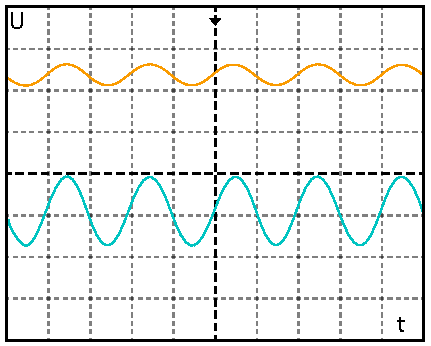
\includegraphics[width=1\linewidth]{12.pdf}}
\caption{Склад системи}
\label{ris1}
\end{figure}


\begin{align}
T_{\text{підх}} = \dfrac{R}{W} = \dfrac{2000}{1,5} = 1333 \text{ }c = 22 \text{ хв}
\end{align}

Через 32 хвилини після аварії хмара зараженого повітря підійде до
населеного пункту. За цей час треба оповістити та евакуювати населення в
безпечний район.
\noindent{\color{babyblue} \rule{\linewidth}{1mm} }

\begin{align}
  t_{\text{ур}} = t_{\text{вип}} = \dfrac{G}{C_{\text{вип}}}
\end{align}


\begin{align}
  t_{\text{вип}} = \dfrac{G}{S}\dfrac{8\cdot 10^{6}}{P_{\text{S}}\cdot \sqrt{M} \cdot (5,38+4,1 \cdot V_{\text{в}}) }\text{хв}
\end{align}\\

$B = \dfrac{G}{\rho} = \dfrac{100 000}{1,42} = 70 422\text{ м}^3$\\

$S = \dfrac{B}{0,05} =\dfrac{70 422}{0,05} = 1 408 450\text{ м}^2$\\


\begin{align}
t_{\text{вип}} = \dfrac{100 000}{1 408 450} \cdot \dfrac{8\cdot 10^{6}}{50\dots 140\cdot \sqrt{M} \cdot (5,38+4,1 \cdot V_{\text{в}})} = 43\dots120  \text{ хв}
\end{align}\\
Таким чином, населений пункт може знаходитись в зоні хімічного
зараження протягом 43 хв. в теплу пору року і протягом 120 хв. -- в холодну пору року.
\noindent{\color{babyblue} \rule{\linewidth}{1mm} }

З табл.1.7(в посібнику) визначаємо, що серед робітників заводу, які забезпечені протигазами на 80\%, очікуються утрати:\\

9\% серед тих, хто буде знаходитись у будівлях;\\

18\% серед тих, хто буде знаходитись на відкритій місцевості.\\

Необхідно забезпечити усіх робітників і службовців заводу
протигазами.






\begin{landscape}

\begin{table}[h]
\begin{center}
\begin{tabular}{|c|c|c|cc|c|c|c|c|}
\hline
\multicolumn{3}{|c|}{Розміри ЗХЗ}   & \multicolumn{2}{c|}{Час підходу, хв}    & \multicolumn{2}{c|}{$\text{Т}_{\text{ур}}$} & \multicolumn{2}{c|}{Утрати, \%} \\ \hline
  Г, км    &   Ш, км   &   S, км$^2$& \multicolumn{2}{c|}{}     &    Взимку       &     Bлітку      &    В будівлях       &      Поза будівлями     \\ \hline
     2,1   &   1,68    &   0,84     & \multicolumn{1}{c}{$43\dots120$}   &          &     43      &    120     &    9     & 18  \\ \hline
\end{tabular}
\end{center}

\caption{Підсумкова таблиця}
\end{table}
\end{landscape}


\end{document}
